\chapter{Requisiti Funzionali}
\label{ch:requisitiFunzionali}

Di seguito vengono riportati i requisiti funzionali (\texttt{RF}) del programma "SatisTrento" tramite \textit{Use Case Diagram} (\texttt{UCD}) progettati usando il linguaggio \texttt{UML}.

% Esempio di markup
\section{\underline{Utente Anonimo}}
    Di seguito i requisiti associati all'Utente Anonimo:
    \begin{itemize}
        \item \textbf{RF1.1}: Visualizzare città
        \item \textbf{RF1.2},\textbf{RF3.1}: Interagire con la Mappa
        \item \textbf{RF2}: Multi lingua
        \item \textbf{RF3.2}: Visualizzare zona
        \item \textbf{RF4}: Accesso dati specifici zona selezionata
        \item \textbf{RF5}: Login
    \end{itemize}
    \begin{figure}[H]
        \centering
        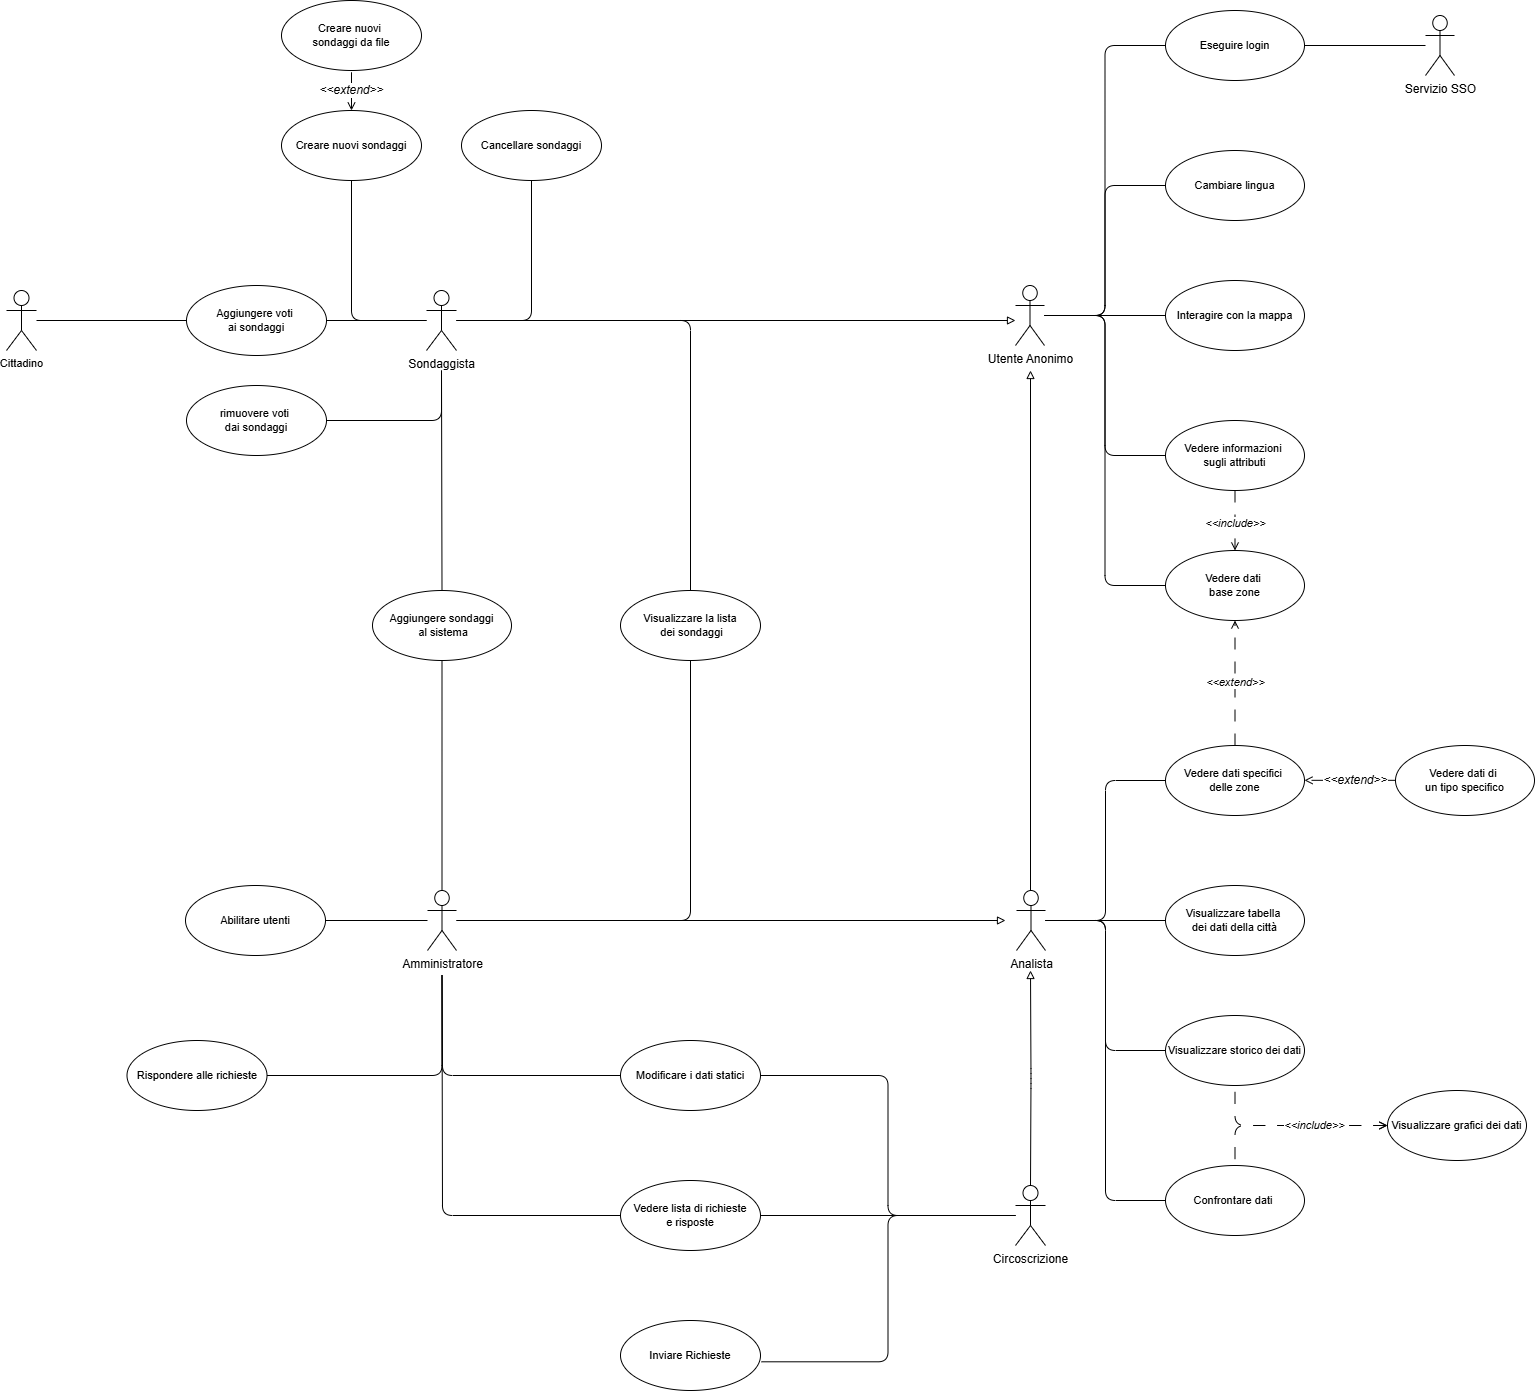
\includegraphics[width=0.8\textwidth]{UseCase_diagrams/Anonimo.drawio.png}
        \caption{Use Case Diagram dell'Utente anonimo}
    \end{figure}

    \subsection{Visualizzare città}
        \subsubsection{Riassunto}
            Questo Use Case descrive come l'utente potrà visualizzare i dati e la mappa della città
        \subsubsection{Descrizione}
            \begin{itemize}
                \item Il sistema mostra nella parte sinistra dello schermo i dati generici della città
                \item Il sistema mostra nella parte destra dello schermo la mappa della città divisa in quartieri
            \end{itemize}
    
    \subsection{Interagire con la Mappa}
        \subsubsection{Riassunto}
            Questo Use Case descrive come l'utente potrà interagire con la mappa
        \subsubsection{Descrizione}
            \begin{itemize} 
                \item L'utente anonimo posiziona il cursone all'interno dello spazio dedicato alla mappa
                \item Se l'utente utilizza la rotella del mouse oppure uno dei pulsanti prensenti in uno degli angoli della mappa
                \item Il sistema ingrandisce o diminuisce la dimensione dello zoom (Eccezione 1)
                \item Se l'utente preme e trascina il cursore
                \item Il sistema sposta il focus centrale all'interno della mappa (Eccezione 2)
                \item Se l'utente anonimo preme una delle zone all'interno della visuale della mappa
                \item Il sistema posiziona il focus centrale della mappa al centro della zona selezionata e ne modifica lo zoom in modo da poter vedere completamente la zona selezionata
                \item Il sistema evidenzia il colore e i bordi della zona selezionata
                \item Il sistema passa allo UseCase "Visualizzazione zona"
            \end{itemize}
        \subsubsection{Eccezioni}
            \begin{enumerate}
                \item Nel caso in cui l'utente anonimo cercasse di aumentare o diminuire lo zoom oltre ai limiti imposti dalla mappa, il sistema deve bloccare la nuova modifica allo zoom
                \item Nel caso in cui l'utente anonimo cercasse di spostare il focus centrale oltre ai limiti della città, il sistema deve bloccare la nuova modifica allo spostamento del focus centrale
            \end{enumerate}
        \subsubsection{Estensioni}
            \begin{enumerate}
                \item Nel caso in cui l'utente cliccasse su di un quartiere già selezionato questo riporterebbe allo UseCase "Visualizzare città"
            \end{enumerate}
            
    \subsection{Multi lingua}
        \subsubsection{Riassunto}
            Questo Use Case descrive come l'utente potrà cambiare la lingua dei vari testi presenti nel programma
        \subsubsection{Descrizione}
            \begin{enumerate}
                \item L'utente preme su una delle bandiere presenti nella header
                \item Il sistema ricarica la pagina selezionata con i testi nella lingua scelta e mette in evidenza la bandiera con la lingua corrente
            \end{enumerate}
        \subsubsection{Eccezioni}
            \begin{enumerate}
                \item Nel caso in cui l'utente anonimo selezionasse la lingua già selezionata, il sistema non deve fare nulla
            \end{enumerate}

    \subsection{Visualizzare zona}
        \subsubsection{Riassunto}
            Questo Use Case descrive come l'utente potrà visualizzare la zona selezionata della città
        \subsubsection{Descrizione}
            \begin{enumerate}
                \item Dopo aver interagito con la mappa ed aver selezionato una zona
                \item Il sistema mostra nella parte sinistra dello schermo la mappa
                \item Il sistema mostra nella parte destra dello schermo i dati generici della zona della città selezionata
            \end{enumerate}

    \subsection{Accesso dati specifici zona selezionata}
        \subsubsection{Riassunto}
            Questo Use Case descrive come l'utente potrà accedere ai dati specifici della zona di preferenza
        \subsubsection{Descrizione}
            \begin{enumerate}
                \item L'utente anonimo preme uno dei dati presenti a schermo
                \item Il sistema presenta a schermo, dove prima erano presenti i vari dati riguardanti la zona selezionata, una tabella con titolo il nome del dato del quale si vuole ricevere un maggior numero di informazioni e contenente tutti gli elementi appartenenti alla specifica del dato scelto (Eccezione 1)
                \item Il sistema deve successivamente segnare sulla mappa la posizione dei vari elementi appartenenti alla specifica del dato scelto con un numero identificativo per identificarne la posizione
            \end{enumerate}
        \subsubsection{Eccezioni}
            \begin{enumerate}
                \item Nel caso in cui per una tipologia di dato non fossero presenti dati specifici il sistema non deve fare nulla
            \end{enumerate}
        \subsubsection{Estensioni}
            \begin{enumerate}
                \item Nel caso in cui l'utente cliccasse il pulante per chiudere la tabella il sistema tornerà alla visualizzazione dei dati della zona selezionata in precedenza
            \end{enumerate}

    \subsection{Login}
        \subsection{Riassunto}
            Questo Use Case descrive come l'utente potrà fare il login
        \subsection{Descrizione}
            \begin{enumerate}
                \item L'utente anonimo preme il pulsante di login presente nella header
                \item Il sistema reindirizza l'utente al sistema SSO
                \item Il sistema SSO verifica l'identità dell'utente in questione e la ritorna al sistema (Eccezione 1)
                \item Il sistema controlla che per l'identità certificata dal sistema SSO esista un'account collegato (Eccezione 1)
                \item Il sistema assegna all'utente anonimo il ruolo posseduto dall'account al quale si è collegato
                \item Il sistema successivamente al login sostituisce l'icona del login con l'immagine profilo dell'account al quale si ha fatto l'accesso
            \end{enumerate}
        \subsection{Eccezioni}
            \begin{enumerate}
                \item Nel caso in cui l'autenticazione fallisse o non vi fossero account collegati il sistema ritorna alla pagina dalla quale si ha provato a fare il login
            \end{enumerate}


\section{\underline{Utente Sondaggista}}
    Di seguito i requisiti associati all'Utente Sondaggista:
    \begin{itemize}
        \item \textbf{RF6}: Logout
        \item \textbf{RF7}: Visualizzazione dati sondaggisti
        \item \textbf{RF8}: Accesso come sondaggista
        \item \textbf{RF9}: Creazione nuovi sondaggi
        \item \textbf{RF10}: Svolgimento sondaggi
    \end{itemize}
    \begin{figure}[H]
        \centering
        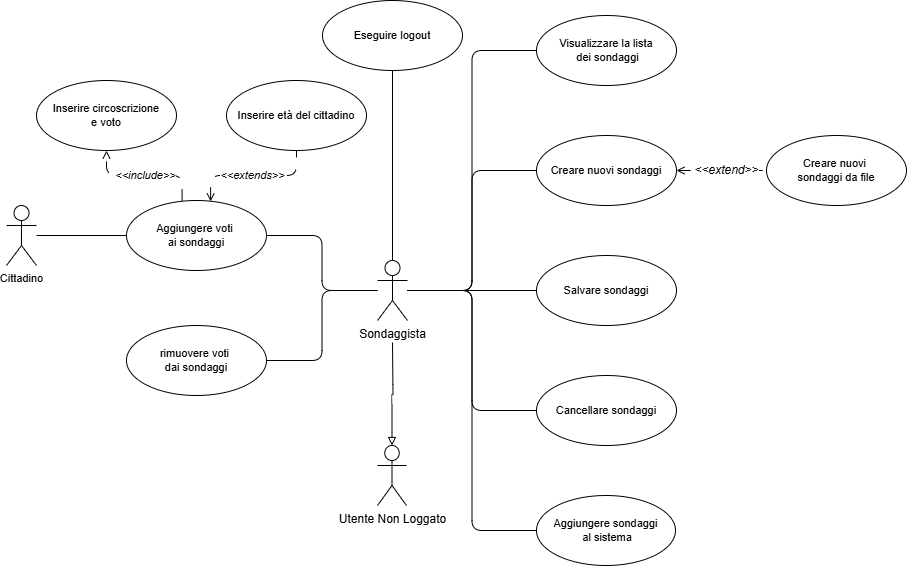
\includegraphics[width=0.8\textwidth]{UseCase_diagrams/Sondaggista.drawio.png}
        \caption{Use Case Diagram dell'Utente sonaggista}
    \end{figure}

    \subsection{Use Case RF6: Logout}
        \subsubsection{Riassunto}
            Questo Use Case descrive come l'utente può fare logout
        \subsubsection{Descrizione}
            \begin{enumerate}
                \item L'utente sondaggista preme sull'icona contenente l'immagine profilo nella header
                \item Il sistema apre un menù a tendina con la sezione 'Logout'
                \item L'utente preme sulla sezione 'Logout'
                \item Il sistema ricarica la pagina riportando l'utente alla 'visualizzazione mappa e dati', scollegandolo dall'account sondaggista al quale era collegato e riportando l'utente allo stato di Utente non loggato
            \end{enumerate}
        \subsubsection{Eccezioni}
            \begin{enumerate}
                \item Nel caso in cui fosse aperta il menù a tendina con la sezione logout e venisse premuto un qualsiasi altro punto sullo schermo il sistema deve chiudere il menù a tendina
            \end{enumerate}
    \subsection{Use Case RF7: Visualizzazione dati sondaggisti}
        \subsection{Titolo}
            Questo Use Case descrive come l'utente sondaggista visualizzerà l'interfaccia per gestire i sondaggi
        \subsection{Descrizione}
            \begin{enumerate}
                \item Il sistema successivamente al login reindirizza l'utente sondaggista alla pagina di gestione dei sondaggi
                \item Il
            \end{enumerate}
        \subsection{Eccezioni}
        \subsection{Estensioni}